% !TeX root = RJwrapper.tex
\title{Conversations in time: interactive visualisation to explore structured
temporal data}
\author{by Earo Wang and Dianne Cook}

\maketitle

\abstract{%
The \pkg{tsibbletalk} package can be used to interactively explore
temporal data of nesting and crossing structures, and discover
interesting periodic/aperiodic slices. This package implements a shared
\texttt{tsibble} object that allows for linked brushing for coordinated
views, and a shiny module that aids in wrapping time lines for seasonal
patterns. The basic usage of functions is demonstrated in the article,
wit data examples.
}

\hypertarget{introduction}{%
\section{Introduction}\label{introduction}}

\begin{itemize}
\tightlist
\item
  An ensemble of graphics
\item
  Accelerate the exploratory data visualisation process
\end{itemize}

\hypertarget{background-tidy-temporal-data-and-workflow}{%
\section{Background: tidy temporal data and
workflow}\label{background-tidy-temporal-data-and-workflow}}

The \CRANpkg{tsibble} package \citep{wang2020tsibble} introduces a
unified temporal data structure, referred to as a \texttt{tsibble}, to
represent time series and longitudinal data in a tidy format
\citep{wickham2014tidy}. That said, a \texttt{tsibble} extends the
\texttt{data.frame} and \CRANpkg{tibble} classes with temporally
contextual metadata: \texttt{index} and \texttt{key}. The \texttt{index}
declares a data column that holds time-related indices. The \texttt{key}
identifies a collection of related series or panels observed over the
\texttt{index}-defined period, which can comprise multiple columns.
Below displays the monthly Australian retail trade turnover data
(\texttt{aus\_retail}), available in the \CRANpkg{tsibbledata} package
\citep{R-tsibbledata}. The \texttt{Month} column holds year-months as
\texttt{index}. The \texttt{State} together with \texttt{Industry} are
the identifiers for these 152 series, highlighted as \texttt{key}. Note
that the column \texttt{Series\ ID} could be an alternative option for
setting up \texttt{key}, but \texttt{State} and \texttt{Industry} are
more readable and informative. The \texttt{index} and \texttt{key} are
``sticky'' columns to a \texttt{tsibble}, forming critical pieces for
fluent temporal data analysis later.

\begin{Schunk}
\begin{Soutput}
#> # A tsibble: 64,532 x 5 [1M]
#> # Key:       State, Industry [152]
#>   State                Industry                    `Series ID`    Month Turnover
#>   <chr>                <chr>                       <chr>          <mth>    <dbl>
#> 1 Australian Capital ~ Cafes, restaurants and cat~ A3349849A   1982 Apr      4.4
#> 2 Australian Capital ~ Cafes, restaurants and cat~ A3349849A   1982 May      3.4
#> 3 Australian Capital ~ Cafes, restaurants and cat~ A3349849A   1982 Jun      3.6
#> 4 Australian Capital ~ Cafes, restaurants and cat~ A3349849A   1982 Jul      4  
#> 5 Australian Capital ~ Cafes, restaurants and cat~ A3349849A   1982 Aug      3.6
#> # ... with 64,527 more rows
\end{Soutput}
\end{Schunk}

In the spirit of tidy data to the \CRANpkg{tidyverse}
\citep{Wickham2019}, the \textbf{tidyverts} suite features
\texttt{tsibble} as the foundational data structure, in order to build a
fluid and fluent pipeline for time series analysis. Besides
\CRANpkg{tsibble}, the \CRANpkg{feasts} \citep{R-feasts} and
\CRANpkg{fable} \citep{R-fable} packages fill the role of statistical
analysis and forecasting in the \textbf{tidyverts} ecosystem. When time
series analysis starts taking off, series of interest denoted by the
\texttt{key} variables often remain unchanged over the course of
analysis, from trend inspection to forecasting performance.

Figure \ref{fig:highlight-retail-1} gives an overview of 152 series for
the retail data using an overlaid time series plot, while Figure
\ref{fig:highlight-retail-2} presents a scatterplot, where each series
is represented by a dot in the feature space (trend versus seasonal
strength). The plot making of Figure \ref{fig:highlight-retail-2} is
aided with the \texttt{features()} function from \CRANpkg{feasts}, which
summarises original data by each series down to various statistical
features. This function along with other \textbf{tidyverts} functions is
\texttt{tsibble}-aware, and outputs a table in a reduced form where each
row corresponds to a series, thus graphically displayed as Figure
\ref{fig:highlight-retail-2}.

\begin{Schunk}
\begin{figure}

{\centering \subfloat[1\label{fig:highlight-retail-1}]{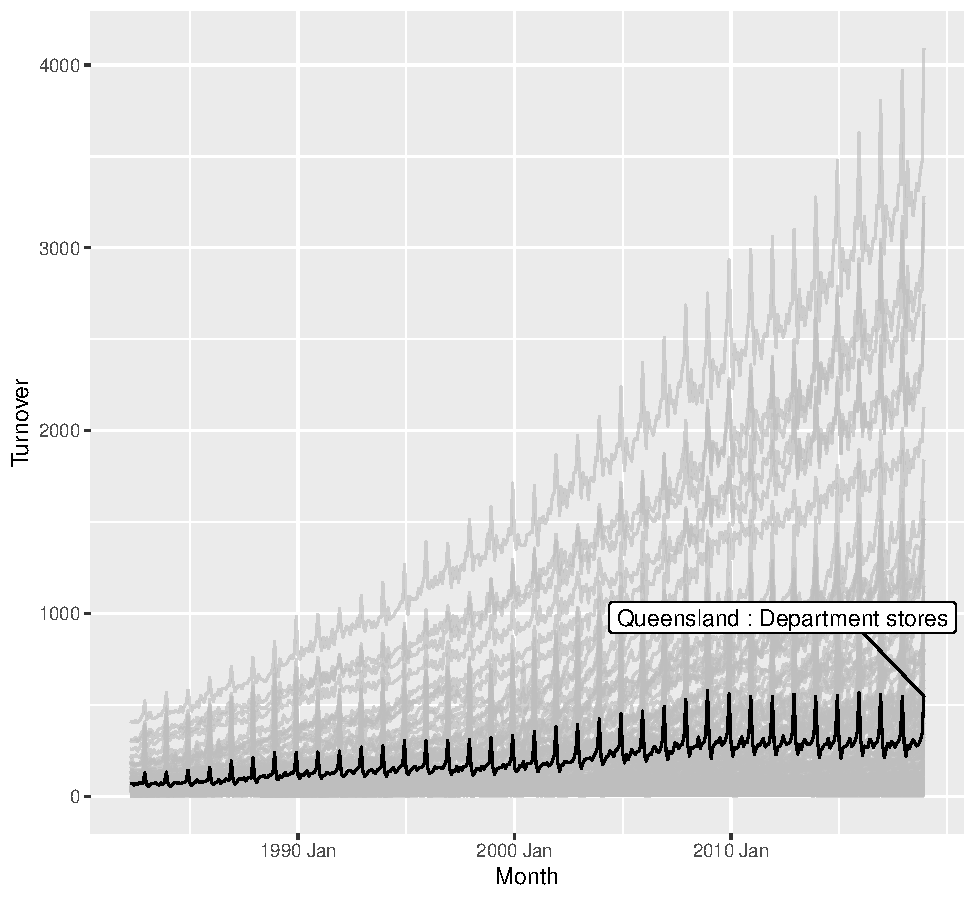
\includegraphics[width=.49\linewidth]{figure/highlight-retail-1} }\subfloat[2\label{fig:highlight-retail-2}]{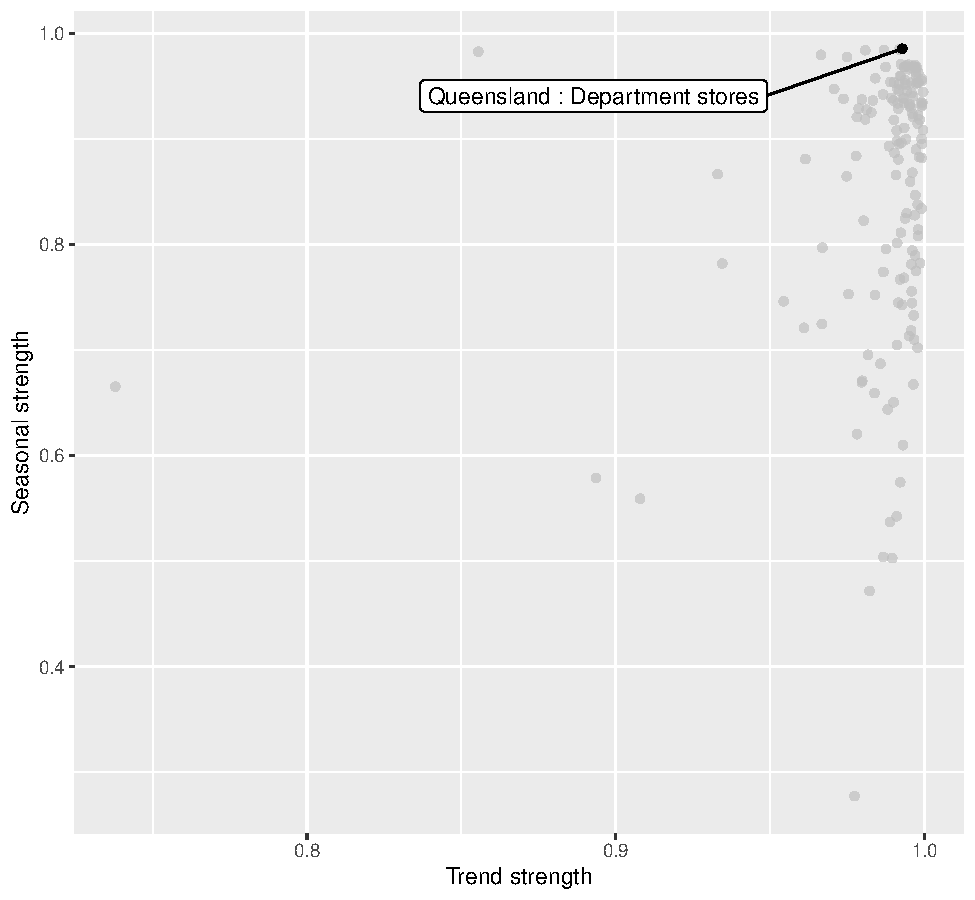
\includegraphics[width=.49\linewidth]{figure/highlight-retail-2} }

}

\caption[ToDo]{ToDo}\label{fig:highlight-retail}
\end{figure}
\end{Schunk}

Figure \ref{fig:highlight-retail} highlights not only a series with
strongest seasonality, but also a need to querying interesting series on
the fly. Without interactivity, one needs to first filter the
interesting series out from the features table, and join back to the
original \texttt{tsibble} in order to examine its trend in relation to
others. This procedure can soon grow cumbersome if many series to be
discovered. Despite that the two plots are static, they can be
considered as linked views via the common \texttt{key} variables between
two tables. This motivates enabling interactivity of \texttt{tsibble}
and \texttt{tsibble}-derived objects for rapid exploratory data
analysis.

\hypertarget{overview-of-interactivity}{%
\section{Overview of interactivity}\label{overview-of-interactivity}}

The R community has a long-standing contribution to interactive
visualisation systems in abundance. These systems can be roughly divided
into two classes: ones with web technology and the others without.

R \CRANpkg{shiny} \citep{R-shiny} and \CRANpkg{htmlwidgets}
\citep{R-htmlwidgets} lay a fundamental infrastructure in marrying R
with HTML elements and Javascript for interactivity, although they
seldom emphasise on interactive graphics. The \CRANpkg{htmlwidgets}
package opens a door to embedding Javascript libraries into R such that
users are able to write only R code to generate web-based plots. Many
Javascript charting libraries have been ported to R as HTML widgets,
including \CRANpkg{plotly} \citep{plotly2020}, \CRANpkg{rbokeh}
\citep{R-rbokeh}, and \CRANpkg{leaflet} \citep{R-leaflet} for maps. To
enable interactions between different widgets, it can be achieved with
\CRANpkg{shiny} or \CRANpkg{crosstalk} \citep{R-crosstalk}. The
\CRANpkg{crosstalk} extends \CRANpkg{htmlwidgets} with shared R6
instances to support linked brushing and filtering across widgets,
without relying on \CRANpkg{shiny}.

If not using web technology, two examples are provided here:
\CRANpkg{loon} \citep{R-loon} based on Tcl/Tk and \pkg{cranvas}
\citep{xie_reactive_2014} based on Qt. They offer a wide array of
pre-defined interactions, such as selecting and zooming, to manipulate
plots via mouse, keyboard strokes, and menus. The \pkg{cranvastime}
package \citep{cheng_enabling_2016} is an add-on of \pkg{cranvas}, which
develops a set of novel interactions for temporal data, for example
wrapping and mirroring.

\hypertarget{interactivity-for-coordinated-views-via-shared-temporal-data}{%
\section{Interactivity for coordinated views via shared temporal
data}\label{interactivity-for-coordinated-views-via-shared-temporal-data}}

The \CRANpkg{tsibbletalk} package, inspired by the \CRANpkg{crosstalk}
package, introduces a shared tsibble instance on top of a
\texttt{tsibble} to allow for frictionless communication between
different plots for temporal data. The \texttt{as\_shared\_tsibble()}
function provides an entry point in the integrated flow, turning a
\texttt{tsibble} to a shared instance (i.e.~\texttt{SharedTsibbleData}
subclassing of \texttt{SharedData} from \CRANpkg{crosstalk}) that powers
data transmission across multiple views. The \CRANpkg{tsibbletalk}
package aims to streamline interactive graphical analysis with the focus
of temporal and structured linking.

As opposed to one-to-one linking, \CRANpkg{tsibbletalk} defaults to
categorical linking where marking one or more observations in one
category will broadcast to all other observations in this category.
Given time series plots, click any data point on a line, highlighting
the whole line as a result. The \texttt{as\_shared\_tsibble()} uses
\texttt{tsibble}'s \texttt{key} variables to achieve these types of
linking, and the \texttt{spec} argument takes one step further in
constructing hybrid linking, such as hierarchical and categorical
linking. For example, each series in the \texttt{aus\_retail} data
corresponds to all possible combinations of the \texttt{State} and
\texttt{Industry} variables. They are intrinsically crossed with each
other. If one variable is nested within another, this lends itself to a
hierarchical structure, like geographical hierarchy. Such collection of
inter-related time series are referred to as hierarchical and grouped
time series in the literature \citep{fpp}.

To incorporate structured specifications in the \texttt{key}, a symbolic
formula can be passed to the \texttt{spec} argument. Adopting Wilkinson
notations for factorial models \citep{Wilkinson1973}, the \texttt{spec}
follows the \texttt{/} and \texttt{*} operators tradition to declare
nesting and crossing variables respectively. The \texttt{spec} for the
\texttt{aus\_retail} data is therefore specified as
\texttt{State\ *\ Industry} or \texttt{Industry\ *\ State}, which is the
default for the presence of multiple \texttt{key} variables. If there is
a hierarchy in the data, using \texttt{/} is required to indicate the
parent-child relation, as strictly one direction \texttt{parent/child}.

The \texttt{tourism\_monthly} dataset \citep{tourism} packaged in
\CRANpkg{tsibbletalk}, contains monthly domestic overnight trips across
Australia, to give an illustrator of nesting and crossing. The
\texttt{key} is comprised of three identifying variables:
\texttt{State}, \texttt{Region}, and \texttt{Purpose} (of trip), in
particular \texttt{State} nesting of \texttt{Region}, together crossed
with \texttt{Purpose}. This specification can be translated as follows:

\begin{Schunk}
\begin{Sinput}
library(tsibbletalk)
tourism_shared <- tourism_monthly %>% 
  as_shared_tsibble(spec = (State / Region) * Purpose)
\end{Sinput}
\end{Schunk}

\begin{Schunk}
\begin{figure}

{\centering 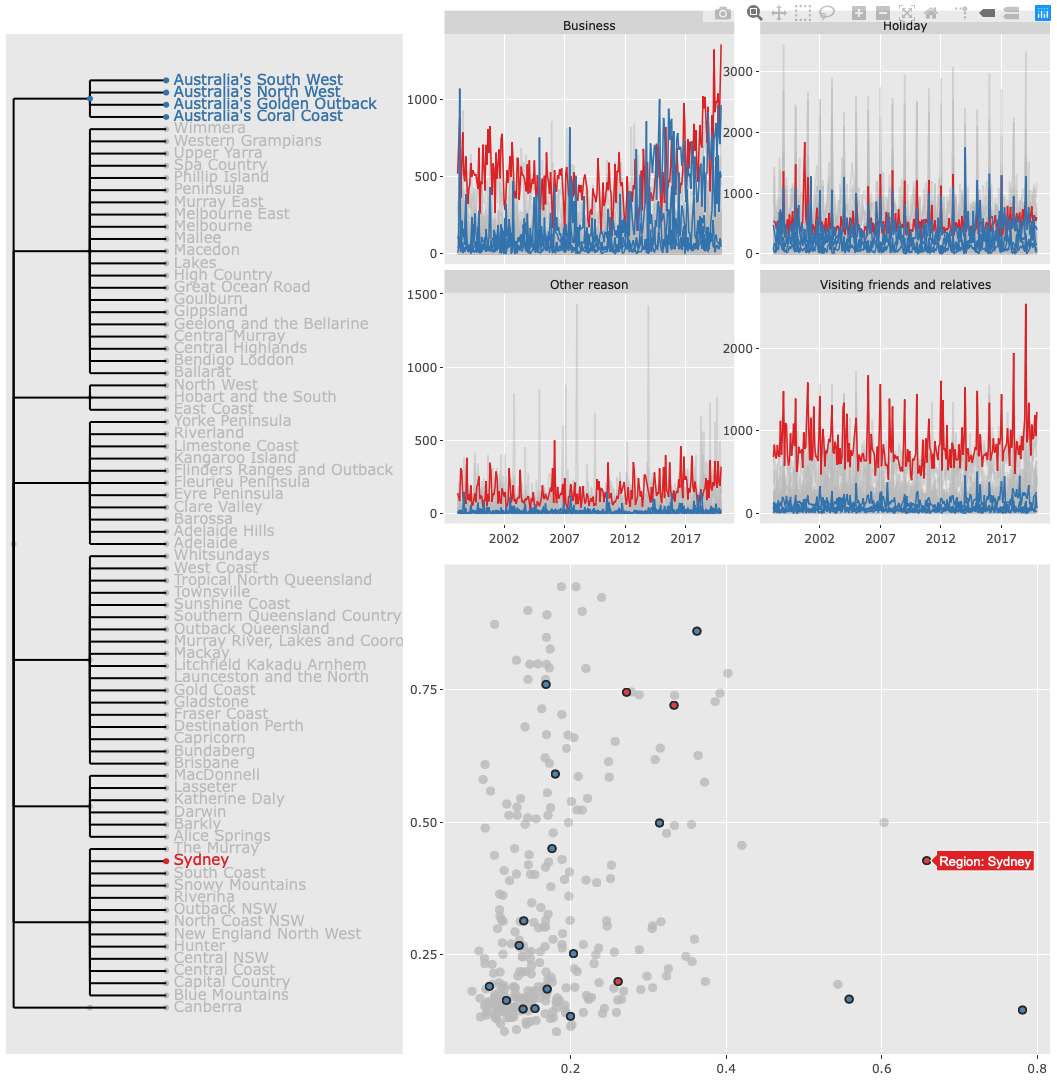
\includegraphics[width=\textwidth]{img/tourism-linking} 

}

\caption[ToDo]{ToDo}\label{fig:tourism-linking-fig}
\end{figure}
\end{Schunk}

This dataset contains a three-level hierarchy: the root node is
implicitly Australia, and geographically disaggregated to states and
lower-level tourism regions. A new handy function
\texttt{plotly\_key\_tree()} has been implemented to address the need of
hierarchical discovery arising from the data. It interprets hierarchies
in the shared tsibble's \texttt{spec} as a tree view, built with
\CRANpkg{plotly}. The following code line produces the linked tree
diagram and fills the left panel of Figure
\ref{fig:tourism-linking-fig}. The visual of tree hierarchy untangles a
group of related series and snapshots the data organisation from a
bird's eye view.

\begin{Schunk}
\begin{Sinput}
p_l <- plotly_key_tree(tourism_shared, height = 1100, width = 800)
\end{Sinput}
\end{Schunk}

The tree plot provides backbones of the data, and much flesh yet to be
attached. Small multiples of time series lines are composed and placed
at the top right of Figure \ref{fig:tourism-linking-fig} to unpack the
temporal trend across regions by purposes of trips. The shared tsibble
data can be directly piped into \CRANpkg{ggplot2} code.

\begin{Schunk}
\begin{Sinput}
p_tr <- tourism_shared %>%
  ggplot(aes(x = Month, y = Trips)) +
  geom_line(aes(group = Region), alpha = .5, size = .4) +
  facet_wrap(~ Purpose, scales = "free_y") +
  scale_x_yearmonth(date_breaks = "5 years", date_labels = "%Y")
\end{Sinput}
\end{Schunk}

To tease apart these overlaid time series, they are funnelled through
the \texttt{features()} S3 method to extract some key characteristics,
including the measurements of trend and seasonality. A scatterplot is
populated from these statistics for each series.

\begin{Schunk}
\begin{Sinput}
tourism_feat <- tourism_shared %>%
  features(Trips, feat_stl)
p_br <- tourism_feat %>%
  ggplot(aes(x = trend_strength, y = seasonal_strength_year)) +
  geom_point(aes(group = Region), alpha = .8, size = 2)
\end{Sinput}
\end{Schunk}

Lastly, three graphics are composed as an ensemble of coordinated views
for multi-facetted exploration, shown as Figure
\ref{fig:tourism-linking-fig} (the interactive realisation of Figure
\ref{fig:highlight-retail}). Routine functions bring about new
interaction with temporal data on the client side.

\begin{Schunk}
\begin{Sinput}
subplot(p_l,
  subplot(
    ggplotly(p_tr, tooltip = "Region", width = 1100),
    ggplotly(p_br, tooltip = "Region", width = 1100),
    nrows = 2),
  widths = c(.4, .6)) %>%
  highlight(dynamic = TRUE)
\end{Sinput}
\end{Schunk}

Since all plots are stemmed from one shared tsibble data source, they
are self-linking views. Nodes, lines, and points are hoverable and
clickable. Given the \texttt{spec}, clicking either one element in any
plot highlights all points that match the \texttt{Region} category,
briefly ``categorical linking''. In Figure
\ref{fig:tourism-linking-fig}, when hovering and selecting the circle
associated with ``Sydney'' in the scatter plot, all data records with
shared values of ``Sydney'' listen and react to this interaction via
self updating in red. In order for comparison with other regions or
states, press the ``Shift'' key to enable persistent selection, and
simultaneously select the parent node on the tree, saying ``Western
Australia'', to include all the children by switching to the blue
colour. The domestic tourism sees Sydney as one of the most popular
destinations in realm of business and friends visiting over years.
Despite of relatively weaker performance in Western Australia,
Australia's North West region sees the strongest upward trend, bypassing
Sydney in some years.

In summary, shared tsibble data nicely bridges between the
\CRANpkg{crosstalk} and \textbf{tidyverts} ecosystems for temporal data
over their common term ``key''. The \texttt{as\_shared\_tsibble()}
provides a symbolic user interface for effortless construction of a
hybrid of hierarchical and categorical linkings. And the
\texttt{plotly\_key\_tree()} in turn decodes the specification to plot a
tree for data overview and navigation, accompanied with more detailed
plots.

\hypertarget{slicing-and-dicing-time}{%
\section{Slicing and dicing time}\label{slicing-and-dicing-time}}

The shared tsibble data leverages the \texttt{key} attribute to converse
with many coordinated views, with or without \CRANpkg{shiny}. On the
other hand, a second critical attribute--\texttt{index}--lays the
foundational temporal context that augments the conversation. When
temporal data are plotted and stretched against the entire span like
Figure \ref{fig:highlight-retail-1}, it puts emphasis on the trend
perception. Yet to digest periodic/aperiodic patterns, data should be
wrapped over relative time units that are origin-less, such as one
quarter or one day.

\begin{Schunk}
\begin{figure}

{\centering \subfloat[(1)\label{fig:wrap-ped-1}]{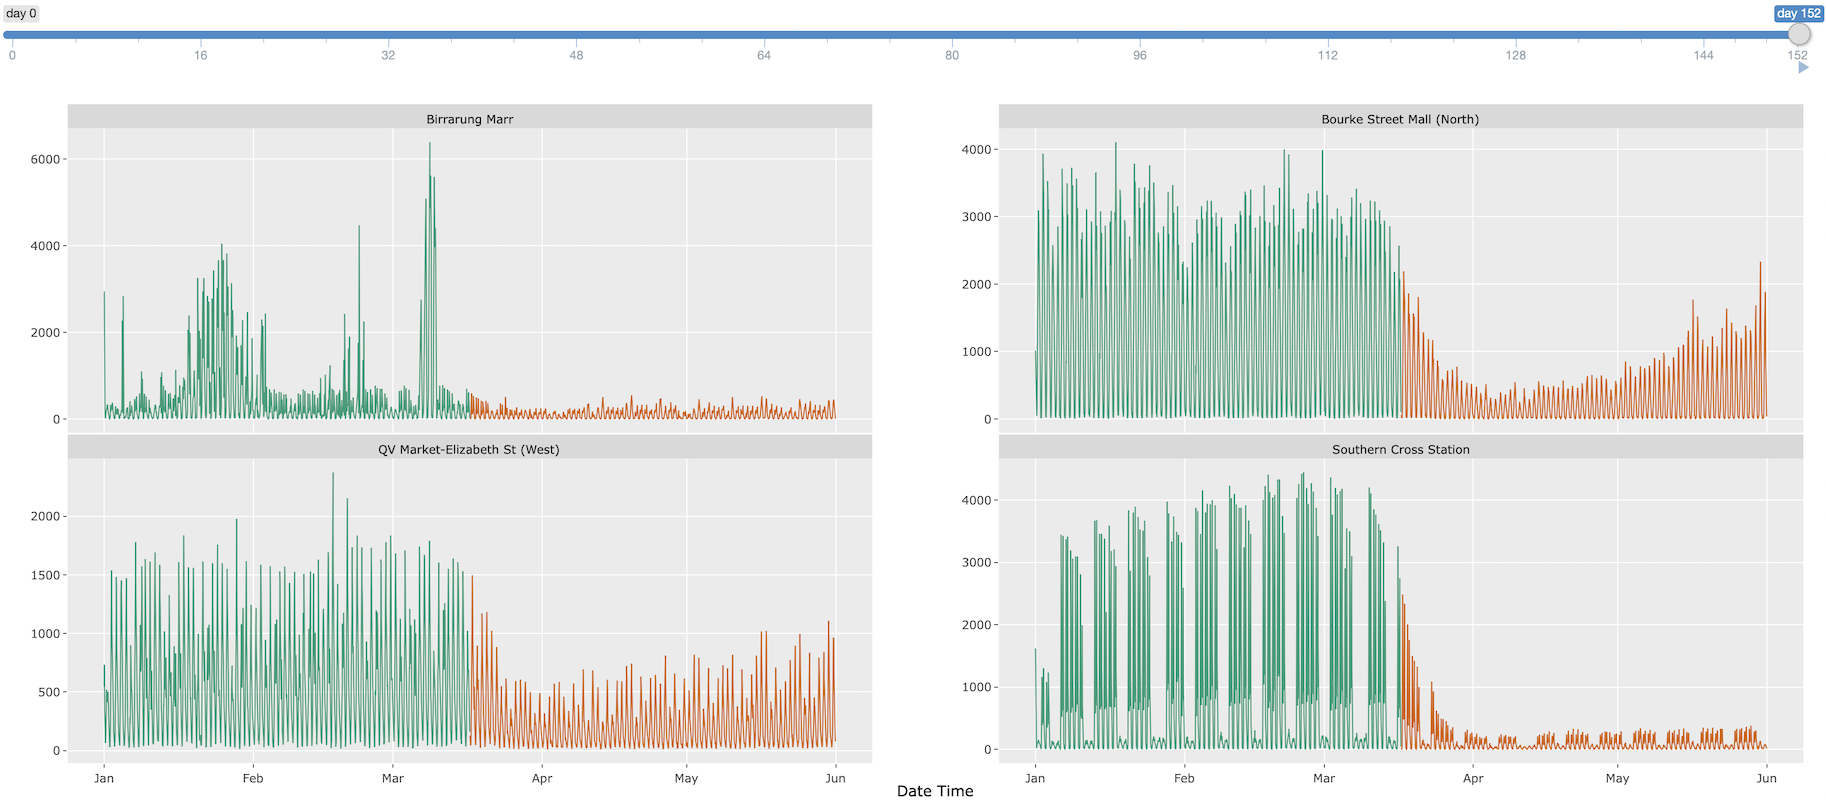
\includegraphics[width=\textwidth]{img/wrap-0} }\newline\subfloat[(2)\label{fig:wrap-ped-2}]{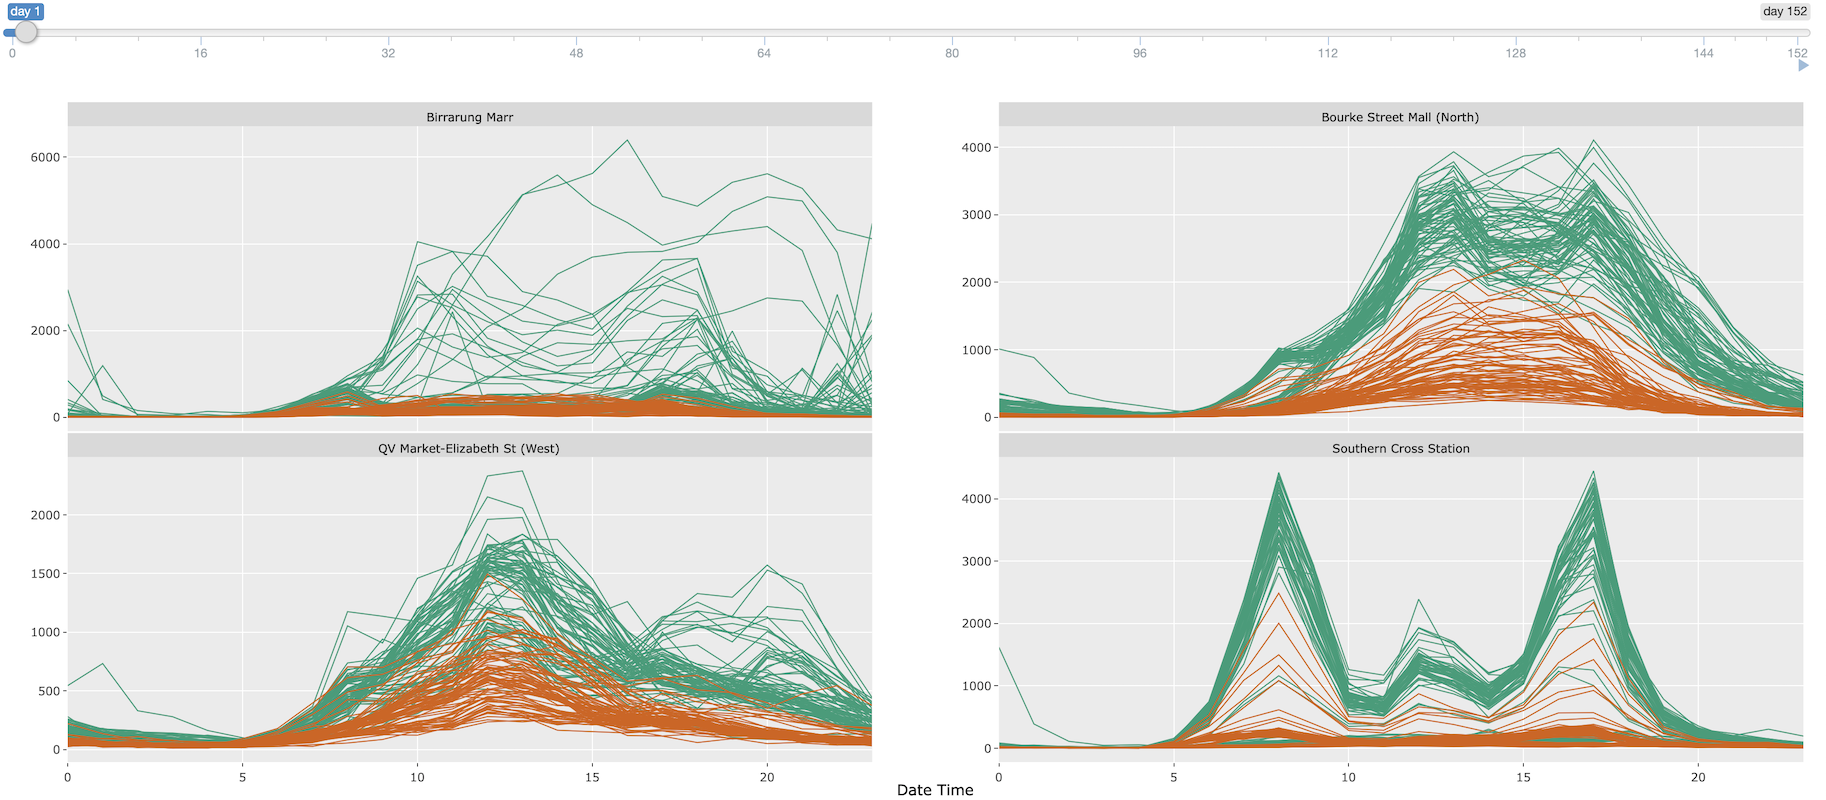
\includegraphics[width=\textwidth]{img/wrap-1} }\newline\subfloat[(3)\label{fig:wrap-ped-3}]{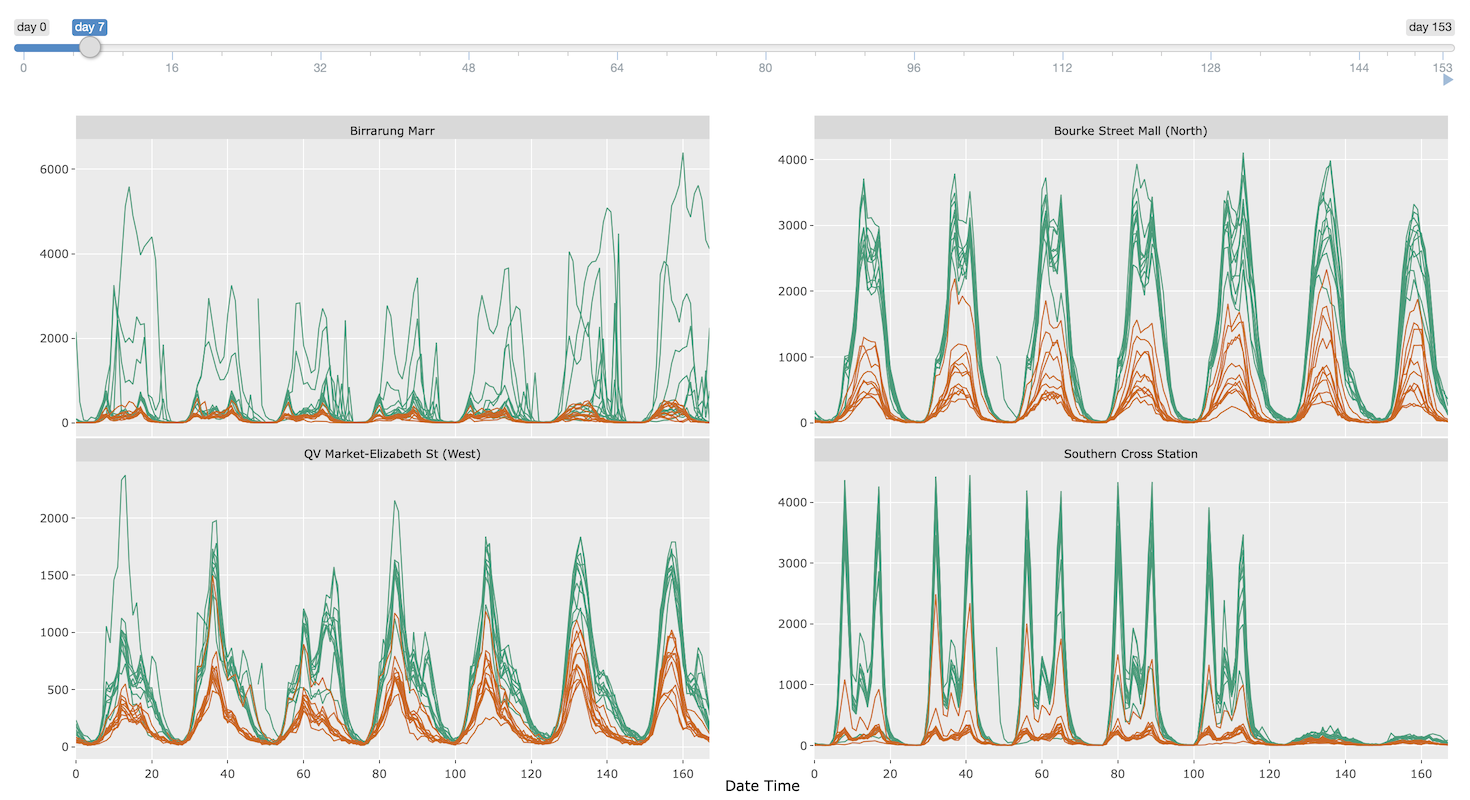
\includegraphics[width=\textwidth]{img/wrap-7} }

}

\caption[ToDo]{ToDo}\label{fig:wrap-ped}
\end{figure}
\end{Schunk}

The city of Melbourne has sensors installed to count hourly tallies of
pedestrians in order to capture downtown daily rhythms \citep{ped}.
Figure \ref{fig:wrap-ped} shows the first five months of 2020 foot
traffic at four locations, with the depiction of three pronounced slices
in time. Figure \ref{fig:wrap-ped-1} unfolds all counts from January to
May on their absolute time line, facetted by four sensors. On March 16,
Melbourne went to the stage three lockdown due to COVID-19, seeing a
significant decline in traffic volume across the city. These lines are
then folded into daily and weekly sections, shown as Figure
\ref{fig:wrap-ped-2} and \ref{fig:wrap-ped-3} respectively. Seasonal
variations have been popped out to viewers, complementing the
not-just-magnitude-drop story. The pre-lockdown period is coloured with
dark green and lockdown with orange.

The wrapping procedure involves slicing time indices into seasonal
periods of interest and their corresponding time dices. For example,
hourly pedestrian data can be decomposed into 24-hour blocks grouped by
all respective days, like Figure \ref{fig:wrap-ped-2}. Figure
\ref{fig:wrap-ped} suggests that there could be more than one
eye-catching slices out of many possible combinations, and thus repeated
wrappings can be unwieldy. To visually locate an interesting slice, the
\CRANpkg{tsibbletalk} package implements a shiny module, a pair of UI
and server functions, to automate this wrapping procedure.

This shiny module, decoupled to \texttt{tsibbleWrapUI()} and
\texttt{tsibbleWrapServer()}, presents a clean interface and forms a
resusable piece in a shiny application. A shiny module provides the
vehicle in modularising shiny applications for both users and
developers. Like all shiny modules, the first argument in both functions
requires a user-supplied session id that must be unique. The UI function
\texttt{tsibbleWrapUI()} simply shows a slider that animates or controls
the number of periods to be diced. The workhorse is certainly the server
function \texttt{tsibbleWrapServer()}, encapsulating the algorithm that
transforms data and sends messages to update the plot accordingly. The
\texttt{plot} argument expects a \texttt{ggplot} or \texttt{plotly}
object, where one can plot data using either lines or other graphical
elements (such as boxplots). As the function name suggests, a (shared)
tsibble is needed to start the engine, and thereby the time
\texttt{index} can be retrieved for dissection. The \texttt{period}
option semantically takes a desired number of seasonal periods to be
shifted, for example data shifted by ``1 day'', ``2 days'', or ``1
week'', etc. In other words, the \texttt{period} defines the grind
level. For date-times (represented by \texttt{POSIXt}), the adjustment
ranges from from fine ``day'' to coarse ``year''. The following code
snippet generates Figure \ref{fig:wrap-ped}.

\begin{Schunk}
\begin{Sinput}
p_line <- pedestrian20 %>%
  ggplot(aes(x = Date_Time, y = Count, colour = Lockdown)) +
  geom_line(size = .3) +
  facet_wrap(~ Sensor, scales = "free_y") +
  labs(x = "Date Time") +
  scale_colour_brewer(palette = "Dark2") +
  theme(legend.position = "none")

ui <- fluidPage(
  tsibbleWrapUI("dice")
)
server <- function(input, output, session) {
  tsibbleWrapServer("dice", ggplotly(p_line, height = 700), period = "1 day")
}
shinyApp(ui, server)
\end{Sinput}
\end{Schunk}

Upon running the shiny application, Figure \ref{fig:wrap-ped-1}
corresponds to the initial state, with the slider incremented by 1-day
unit. The ``play'' button near the end of slider begins animating the
slicing and dicing process by walking through all 24 hours by 153 days.
Alternatively, users can drag the handler to poke around certain slices
themselves.

In response to the slider input, the plot will be updated and loaded
with newly transformed data. At its core, keeping the application as
performant as possible is the top priority. Without completely redrawing
the plot, the \texttt{plotly.js} react method is invoked internally. The
underlying tsibble data is being called back and processed in R. Only
transformed data gets fed back to the shiny server, along with reseting
the x-axis ranges and breaks. The rest plot configurations, such as
marks, y-axes, and layouts, are properly cached.

The new shiny module exploits the temporal aspect for a tsibble object.
It allows users to slide through relative periods to explore seasonal
insights, with slick user experience.

\hypertarget{conclusions-and-discussions}{%
\section{Conclusions and
discussions}\label{conclusions-and-discussions}}

\bibliography{tsibbletalk.bib}

\address{%
Earo Wang\\
The University of Auckland\\%
Auckland, New Zealand\\
%
%
%
\\\href{mailto:earo.wang@auckland.ac.nz}{\nolinkurl{earo.wang@auckland.ac.nz}}
}

\address{%
Dianne Cook\\
Monash University\\%
Melbourne, Australia\\
%
%
%
\\\href{mailto:dicook@monash.edu}{\nolinkurl{dicook@monash.edu}}
}

